% ============================================================
%  research_report.tex
%  Air Quality Analysis Across Indian States:
%    Pollutant Distribution, Socioeconomic Correlates,
%    and Predictive Modelling
%
%  Author : Sayon Mitra
%           UID: 25lbcs1407
%           B.Tech CSE, Chandigarh University
%           Uttar Pradesh, India
%
%  Format : IEEE Transactions / Conference (two-column)
%  Compile: pdflatex -> bibtex -> pdflatex -> pdflatex
% ============================================================

\documentclass[10pt, conference]{IEEEtran}

% ── Encoding & fonts ────────────────────────────────────────
\usepackage[T1]{fontenc}
\usepackage[utf8]{inputenc}

% ── Mathematics ──────────────────────────────────────────────
\usepackage{amsmath, amssymb}

% ── Graphics & tables ────────────────────────────────────────
\usepackage{graphicx}
\usepackage{booktabs}
\usepackage{multirow}
\usepackage{array}
\usepackage{tabularx}

% ── Hyperlinks (remove coloured boxes in print) ──────────────
\usepackage[hidelinks]{hyperref}

% ── Units (µg/m³ etc.) ───────────────────────────────────────
\usepackage{siunitx}
\sisetup{detect-all}

% ── Algorithms / code ────────────────────────────────────────
\usepackage{listings}
\lstset{
  basicstyle=\ttfamily\scriptsize,
  breaklines=true,
  frame=single,
  captionpos=b
}

% ── Miscellaneous ────────────────────────────────────────────
\usepackage{cite}
\usepackage{url}
\usepackage{xcolor}
\usepackage{balance}   % balance columns on last page

% ── Figure path ──────────────────────────────────────────────
\graphicspath{{./}}

% ============================================================
%  TITLE & AUTHORS
% ============================================================
\title{Air Quality Analysis Across Indian States:\\
Pollutant Distribution, Socioeconomic Correlates,\\
and Predictive Modelling}

\author{
  \IEEEauthorblockN{Sayon Mitra}
  \IEEEauthorblockA{
    \textit{B.Tech Computer Science and Engineering}\\
    \textit{Chandigarh University}\\
    Uttar Pradesh, India\\
    UID: 25LBCS1407\\
    \href{mailto:25lbcs1407@culkomail.in}{25lbcs1407@culkomail.in}\\
    \href{mailto:sayon@sayonedu.in}{sayon@sayonedu.in}
  }
}

% ============================================================
\begin{document}
\maketitle

% ============================================================
%  ABSTRACT
% ============================================================
\begin{abstract}
Air pollution is a critical public health and policy challenge
in India, where rapid urbanisation and industrial growth have
placed acute pressure on ambient air quality.
This study analyses real-time pollutant concentration data
from the Central Pollution Control Board (CPCB) monitoring
network, integrating findings with state-level socioeconomic
and health indicators drawn from the National Family Health
Survey (NFHS-5, 2019--21).
Seven major pollutants --- PM$_{10}$, PM$_{2.5}$, CO,
NO$_{2}$, NH$_{3}$, O$_3$, and SO$_{2}$ --- were examined
across 3{,}273 valid monitoring observations spanning 29
states and 267 cities.
Key findings indicate that particulate matter dominates the
pollution landscape, with mean PM$_{10}$ and PM$_{2.5}$
concentrations of 96.11~\si{\micro g/m^3} and
76.60~\si{\micro g/m^3}, respectively --- exceeding WHO
annual guideline values by six- and fifteenfold.
Delhi, Himachal Pradesh, and Jharkhand recorded the highest
composite pollution averages.
Pearson correlation analysis with 29 matched state-level
profiles reveals that infant and under-five mortality are the
only indicators reaching statistical significance
($r = {+}0.45$, $p = 0.017$), while development indicators
show weak inverse trends.
K-Means clustering identified three distinct
pollution-vulnerability state profiles.
Predictive modelling via Pipeline-based cross-validation
confirms that socioeconomic proxies alone are insufficient
for reliable state-level pollution prediction at $n = 29$,
pointing to the need for longitudinal city-level panel data.
The study contributes an integrated, reproducible analytical
framework applicable to future large-scale air quality
research in low- and middle-income country contexts.
\end{abstract}

\begin{IEEEkeywords}
Air Quality Index, PM$_{2.5}$, PM$_{10}$, India, NFHS-5,
K-Means Clustering, Random Forest, Socioeconomic Indicators,
CPCB, Predictive Modelling
\end{IEEEkeywords}

% ============================================================
%  1. INTRODUCTION
% ============================================================
\section{Introduction}
\label{sec:intro}

India's air quality crisis has intensified over the past two
decades, driven by a complex interplay of industrial
emissions, vehicular exhaust, agricultural burning, and
household fuel use~\cite{balakrishnan2019}.
The Global Burden of Disease study estimates that ambient and
household air pollution together account for over 1.6~million
deaths annually in India~\cite{hei2020}.
Despite significant regulatory effort --- including the
National Clean Air Programme (NCAP) launched in 2019 ---
comprehensive, state-level evidence on pollution distribution
and its socioeconomic determinants remains fragmented.

Two primary data resources enable this analysis.
The Central Pollution Control Board (CPCB) operates a
real-time Continuous Ambient Air Quality Monitoring (CAAQM)
network covering hundreds of monitoring stations across India.
The National Family Health Survey (NFHS-5), conducted by the
Ministry of Health and Family Welfare in 2019--21, provides a
rich repository of household-level socioeconomic, health, and
demographic indicators for all states and union territories.

Prior studies have examined individual pollutants~\cite{kumar2015},
city-level AQI trends~\cite{garg2021}, or isolated health
correlates~\cite{landrigan2018}, but few have systematically
integrated CPCB real-time data with NFHS-5 socioeconomic
profiles at the state level.
This study addresses that gap with the following objectives:

\begin{enumerate}[leftmargin=*]
  \item \textbf{Characterise} the distribution of seven key
        pollutants across Indian states and classify
        monitoring readings by standard CPCB AQI categories.
  \item \textbf{Identify} socioeconomic and health indicators
        most strongly correlated with state-level pollution
        exposure.
  \item \textbf{Cluster} states into distinct
        pollution-vulnerability profiles using K-Means
        clustering.
  \item \textbf{Build and evaluate} predictive models for
        state-level mean pollution using socioeconomic
        features, identifying the principal determinants.
\end{enumerate}

The remainder of the paper is structured as follows.
Section~\ref{sec:data} describes the datasets.
Section~\ref{sec:method} details the methodology.
Section~\ref{sec:results} presents results and discussion.
Section~\ref{sec:conclusion} concludes with limitations and
future work.

% ============================================================
%  2. DATASET DESCRIPTION
% ============================================================
\section{Dataset Description}
\label{sec:data}

\subsection{CPCB AQI Dataset (\texttt{aqi.csv})}

The AQI dataset was sourced from the Government of India's
open data portal (\url{data.gov.in}) and represents
real-time readings from CPCB's CAAQM network.
It contains 3{,}411 observations across 11 variables.
Table~\ref{tab:aqi_vars} summarises the key variables.

\begin{table}[htbp]
  \centering
  \caption{CPCB AQI Dataset Variables}
  \label{tab:aqi_vars}
  \renewcommand{\arraystretch}{1.15}
  \begin{tabularx}{\linewidth}{@{}lX@{}}
    \toprule
    \textbf{Variable} & \textbf{Description} \\
    \midrule
    \texttt{state}         & State / union territory name \\
    \texttt{city}          & City of the monitoring station \\
    \texttt{station}       & Full station name (operator) \\
    \texttt{last\_update}  & Timestamp (DD-MM-YYYY HH:MM:SS) \\
    \texttt{latitude/longitude} & Geographic coordinates \\
    \texttt{pollutant\_id} & Pollutant type (PM$_{10}$, PM$_{2.5}$, CO, NO$_2$, NH$_3$, O$_3$, SO$_2$) \\
    \texttt{pollutant\_min/max} & Min/max in reporting window \\
    \texttt{pollutant\_avg} & Mean reading (primary variable) \\
    \bottomrule
  \end{tabularx}
\end{table}

\noindent\textbf{Coverage:} 29 states, 267 cities, 7 pollutants.
The dataset snapshot is dated 27~March~2026 (UTC+5:30).
It contains 138~rows ($\approx$4\%) with \texttt{pollutant\_avg}
reported as \texttt{NA}, which were excluded, leaving
3{,}273 valid observations.

\subsection{NFHS-5 Health and Socioeconomic Dataset (\texttt{health.xls})}

This dataset contains 111~rows and 136~columns representing
state-level NFHS-5 indicator estimates.
Each state has three rows corresponding to Urban, Rural, and
Total (combined) population strata.
Total-stratum rows were retained for state-level analysis.
The dataset covers 37 states and union territories with
socioeconomic, health, education, sanitation, and demographic
indicators~\cite{nfhs5}.

\subsection{Dataset Integration}

State names in the CPCB dataset use underscores as word
separators (e.g., \texttt{Andhra\_Pradesh}), while NFHS-5
uses spaces (\texttt{Andhra Pradesh}).
After normalising both sources to lowercase, replacing
underscores with spaces, and applying a targeted
name-harmonisation dictionary for four residual mismatches
(``NCT of Delhi''~$\rightarrow$~``delhi'';
``Maharastra''~$\rightarrow$~``maharashtra'';
``Andaman \& Nicobar Islands''~$\rightarrow$~``andaman and
nicobar''; ``Jammu \& Kashmir''~$\rightarrow$~``jammu and
kashmir''), a total of \textbf{29 states and union
territories} were successfully matched and merged.
The eight unmatched NFHS territories (Goa, Manipur, Meghalaya,
Ladakh, Lakshadweep, Dadra and Nagar Haveli \& Daman and
Diu, Andaman and Nicobar, India-aggregate) lack corresponding
CPCB monitoring stations in the current snapshot.

% ============================================================
%  3. METHODOLOGY
% ============================================================
\section{Methodology}
\label{sec:method}

\subsection{Data Preprocessing}

\textbf{AQI data.}
Rows with \texttt{pollutant\_avg} equal to \texttt{NA} were
dropped (138~rows; 4.0\%).
State names were normalised to lowercase with underscores
replaced by spaces; a single-entry replacement maps
\texttt{tamilnadu} (CPCB raw) to \texttt{tamil nadu}
(standard).
A composite state-level measure --- the arithmetic mean of
all \texttt{pollutant\_avg} readings across pollutants,
cities, and stations within each state ---
(\texttt{mean\_pollutant\_avg}) was computed to capture the
overall pollution burden.

\textbf{Health data.}
Only ``Total'' (combined urban+rural) rows were retained.
Fourteen columns containing mixed text/numeric data were
coerced to numeric type using
\texttt{pd.to\_numeric(\ldots, errors=`coerce')}.
After name harmonisation, the merged dataset contained
29~state-level observations.

\textbf{AQI categorisation.}
Each pollutant reading was classified using standard CPCB
sub-index thresholds: Good (0--50), Satisfactory (51--100),
Moderate (101--200), Poor (201--300), Very Poor (301--400),
and Severe ($>$400).

\subsection{Statistical Analysis}

Pearson correlation coefficients and associated two-tailed
$p$-values were computed between \texttt{mean\_pollutant\_avg}
and ten selected socioeconomic/health indicators.
Statistical significance was assessed at $\alpha = 0.05$
(critical $|r| \approx 0.37$ for $n = 29$).

\subsection{K-Means Clustering}

K-Means clustering was applied to four variables:
\texttt{mean\_pollutant\_avg}, electricity access, improved
sanitation, and female education --- all standardised using
z-score normalisation (\texttt{StandardScaler}).
The optimal number of clusters was identified via the Elbow
Method (evaluating inertia for $k = 2$ to $7$).
Clusters were visualised by projecting onto the
pollution-vs.-female education axes.

\subsection{Predictive Modelling}

Eight socioeconomic features were used as predictors of
\texttt{mean\_pollutant\_avg}:
(1)~female school attendance (\%),
(2)~electricity access (\%),
(3)~improved sanitation (\%),
(4)~clean cooking fuel (\%),
(5)~women's literacy (\%),
(6)~women with $\geq$10~years schooling (\%),
(7)~tobacco use --- men (\%), and
(8)~alcohol use --- men (\%).

Four regression models were evaluated: Linear Regression
(OLS), Ridge Regression ($\alpha = 1.0$), Random Forest
(200~trees, \texttt{max\_depth}~=~4), and Gradient Boosting
(200~estimators, \texttt{max\_depth}~=~3).

All models were implemented as scikit-learn \texttt{Pipeline}
objects~\cite{pedregosa2011} with \texttt{StandardScaler} as
the first step, ensuring the scaler is re-fitted independently
within each cross-validation fold and eliminating data
leakage.
Data were split 80/20 (train/test) with random seed~42.
Five-fold cross-validation $R^2$ (CV~$R^2$) was computed for
each pipeline.
Performance metrics include MAE, RMSE, test~$R^2$, and
CV~$R^2$.

% ============================================================
%  4. RESULTS AND DISCUSSION
% ============================================================
\section{Results and Discussion}
\label{sec:results}

\subsection{Pollutant Distribution}

Table~\ref{tab:pollutant_stats} summarises descriptive
statistics for each pollutant.

\begin{table}[htbp]
  \centering
  \caption{Descriptive Statistics of Pollutant Average
           Concentrations (\si{\micro g/m^3} or ppb)}
  \label{tab:pollutant_stats}
  \renewcommand{\arraystretch}{1.1}
  \begin{tabular}{@{}lrrrrrr@{}}
    \toprule
    \textbf{Pollutant} & \textbf{n} & \textbf{Mean} & \textbf{Median}
      & \textbf{SD} & \textbf{Min} & \textbf{Max} \\
    \midrule
    PM$_{10}$  & 482 & 96.11 & 91.0 & 38.07 & 23.0 & 268.0 \\
    PM$_{2.5}$ & 486 & 76.60 & 65.0 & 41.30 &  2.0 & 243.0 \\
    CO         & 477 & 35.91 & 32.0 & 22.26 &  2.0 & 131.0 \\
    NO$_2$     & 481 & 29.22 & 24.0 & 21.64 &  1.0 & 138.0 \\
    O$_3$      & 459 & 21.95 & 18.0 & 15.87 &  1.0 & 143.0 \\
    SO$_2$     & 461 & 16.98 & 13.0 & 14.93 &  1.0 & 111.0 \\
    NH$_3$     & 427 &  6.16 &  5.0 &  4.67 &  1.0 &  44.0 \\
    \bottomrule
  \end{tabular}
\end{table}

Particulate matter constitutes the primary pollution concern.
Mean PM$_{10}$ (96.11~\si{\micro g/m^3}) exceeds the WHO
annual guideline (15~\si{\micro g/m^3})~\cite{who2021} by
more than sixfold.
Mean PM$_{2.5}$ (76.60~\si{\micro g/m^3}) exceeds the WHO
guideline (5~\si{\micro g/m^3}) by over fifteenfold.
All pollutants exhibit right-skewed distributions (means
exceed medians), indicating hotspot stations driving the
upper tail.
Figure~\ref{fig:pollutant_dist} illustrates these distributions.

\begin{figure}[htbp]
  \centering
  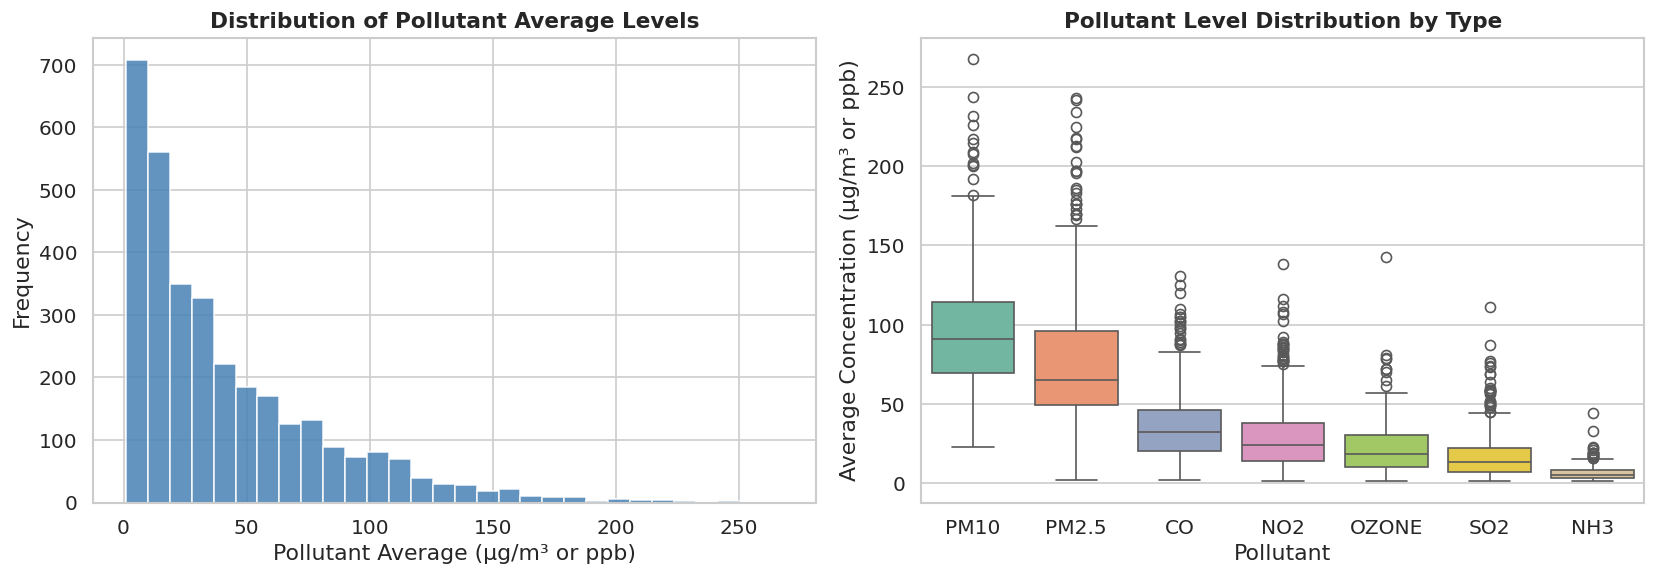
\includegraphics[width=\linewidth]{fig1_pollutant_distribution}
  \caption{Distribution of pollutant average levels:
           (left)~frequency histogram across all readings;
           (right)~box-plots by pollutant type.}
  \label{fig:pollutant_dist}
\end{figure}

\subsection{AQI Category Distribution}

Table~\ref{tab:aqi_cat} shows the breakdown of monitoring
readings by CPCB AQI category.

\begin{table}[htbp]
  \centering
  \caption{Distribution of Monitoring Readings by AQI Category
           ($n = 3{,}273$)}
  \label{tab:aqi_cat}
  \renewcommand{\arraystretch}{1.1}
  \begin{tabular}{@{}lrr@{}}
    \toprule
    \textbf{Category} & \textbf{Count} & \textbf{Share (\%)} \\
    \midrule
    Good          & 2{,}268 & 69.3 \\
    Satisfactory  &     687 & 21.0 \\
    Moderate      &     299 &  9.1 \\
    Poor          &      19 &  0.6 \\
    Very Poor     &       0 &  0.0 \\
    Severe        &       0 &  0.0 \\
    \bottomrule
  \end{tabular}
\end{table}

While 69\% of sub-index readings fall in the ``Good''
category --- reflecting the inclusion of low-concentration
pollutants (NH$_3$, SO$_2$) at baseline levels --- the 9.7\%
at ``Moderate'' or worse represent significant public health
exposure across large urban populations.
It is important to note that these are individual
pollutant sub-index readings, not composite AQI values; the
composite AQI is defined as the maximum sub-index and would
yield a higher share of elevated categories.

\subsection{State-Level Pollution Rankings}

Table~\ref{tab:state_rank} presents the top-10 and bottom-5
states by mean composite pollution level.

\begin{table}[htbp]
  \centering
  \caption{State-Level Mean Composite Pollution Rankings
           (\si{\micro g/m^3} or ppb)}
  \label{tab:state_rank}
  \renewcommand{\arraystretch}{1.1}
  \begin{tabular}{@{}clr@{}}
    \toprule
    \textbf{Rank} & \textbf{State} & \textbf{Mean} \\
    \midrule
    1  & Delhi           & 64.55 \\
    2  & Himachal Pradesh& 61.29 \\
    3  & Tripura         & 53.00 \\
    4  & Jharkhand       & 52.75 \\
    5  & Haryana         & 48.24 \\
    6  & Odisha          & 46.27 \\
    7  & Gujarat         & 44.59 \\
    8  & Punjab          & 43.74 \\
    9  & Uttar Pradesh   & 43.58 \\
    10 & Madhya Pradesh  & 43.13 \\
    \midrule
    25 & Puducherry      & 22.00 \\
    26 & Uttarakhand     & 20.67 \\
    27 & Jammu \& Kashmir& 20.42 \\
    28 & Nagaland        & 17.57 \\
    29 & Sikkim          & 15.71 \\
    \bottomrule
  \end{tabular}
\end{table}

Delhi's position at the top is consistent with established
literature on the National Capital Region's severe air
quality challenges~\cite{chowdhury2016}.
Northern and eastern industrial states (Jharkhand, Haryana,
Odisha) cluster in the high-pollution tier, while smaller
north-eastern states and Himalayan union territories show
consistently lower composite levels.
Figure~\ref{fig:top_states} provides a visual overview.

\begin{figure}[htbp]
  \centering
  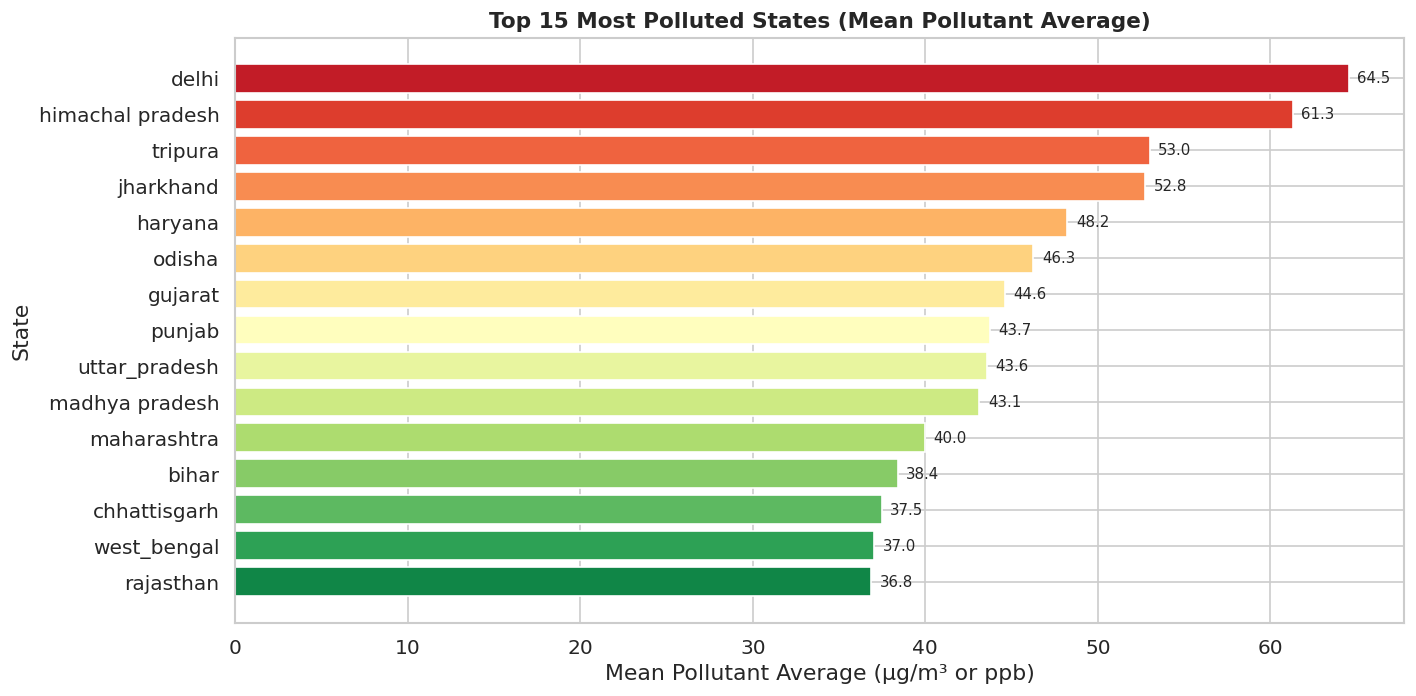
\includegraphics[width=\linewidth]{fig2_top_polluted_states}
  \caption{Top 15 most polluted states by mean composite
           pollutant average (\si{\micro g/m^3} or ppb).}
  \label{fig:top_states}
\end{figure}

\subsection{Correlation Analysis}

Table~\ref{tab:corr} reports Pearson $r$ and two-tailed
$p$-values for ten socioeconomic/health indicators
($n = 29$ states).

\begin{table}[htbp]
  \centering
  \caption{Pearson Correlation with Mean Pollutant Average
           ($n = 29$, critical $|r| \approx 0.37$ at $\alpha=0.05$)}
  \label{tab:corr}
  \renewcommand{\arraystretch}{1.1}
  \begin{tabular}{@{}lrrl@{}}
    \toprule
    \textbf{Indicator} & \textbf{$r$} & \textbf{$p$} & \textbf{Sig.} \\
    \midrule
    Female Education (\%)         & $-0.18$ & 0.353 & --- \\
    Electricity Access (\%)       & $-0.13$ & 0.519 & --- \\
    Improved Sanitation (\%)      & $-0.34$ & 0.069 & $\dagger$ \\
    Clean Cooking Fuel (\%)       & $-0.24$ & 0.215 & --- \\
    Women Literacy (\%)           & $-0.18$ & 0.350 & --- \\
    Women Schooling $\geq$10yr (\%)& $-0.15$ & 0.438 & --- \\
    Tobacco Use --- Men (\%)      & $+0.03$ & 0.859 & --- \\
    Alcohol Use --- Men (\%)      & $-0.10$ & 0.620 & --- \\
    Infant Mortality (per 1{,}000) & $\mathbf{+0.45}$ & $\mathbf{0.017}$ & $*$ \\
    Under-5 Mortality (per 1{,}000)& $\mathbf{+0.44}$ & $\mathbf{0.021}$ & $*$ \\
    \bottomrule
    \multicolumn{4}{@{}l}{\footnotesize
      $*\ p < 0.05$;\quad $\dagger\ p < 0.10$}
  \end{tabular}
\end{table}

Infant mortality ($r = {+}0.45$, $p = 0.017$) and under-five
mortality ($r = {+}0.44$, $p = 0.021$) are the only
indicators reaching conventional statistical significance.
These positive associations suggest that states bearing
higher composite pollution burdens also tend to have higher
child mortality rates --- consistent with the substantial
literature linking particulate matter exposure to adverse
perinatal and early-childhood health
outcomes~\cite{landrigan2018}.
Improved sanitation shows a near-significant negative
correlation ($r = {-}0.34$, $p = 0.069$).

Development indicators (female education, electricity access,
clean cooking fuel) exhibit weak negative correlations,
though none reach significance at $n = 29$.
Three important caveats apply:
(a)~urbanisation acts as a confounder --- Delhi ranks high in
both infrastructure metrics and pollution, attenuating
negative correlations;
(b)~the ecological fallacy applies --- state-level aggregates
mask within-state heterogeneity between urban hotspots and
cleaner rural areas;
(c)~temporal mismatch exists between the CPCB snapshot
(March~2026) and NFHS-5 data (2019--21).
These results are therefore interpreted as exploratory
associations rather than confirmed causal relationships.
Figure~\ref{fig:corr_matrix} shows the full correlation matrix.

\begin{figure}[htbp]
  \centering
  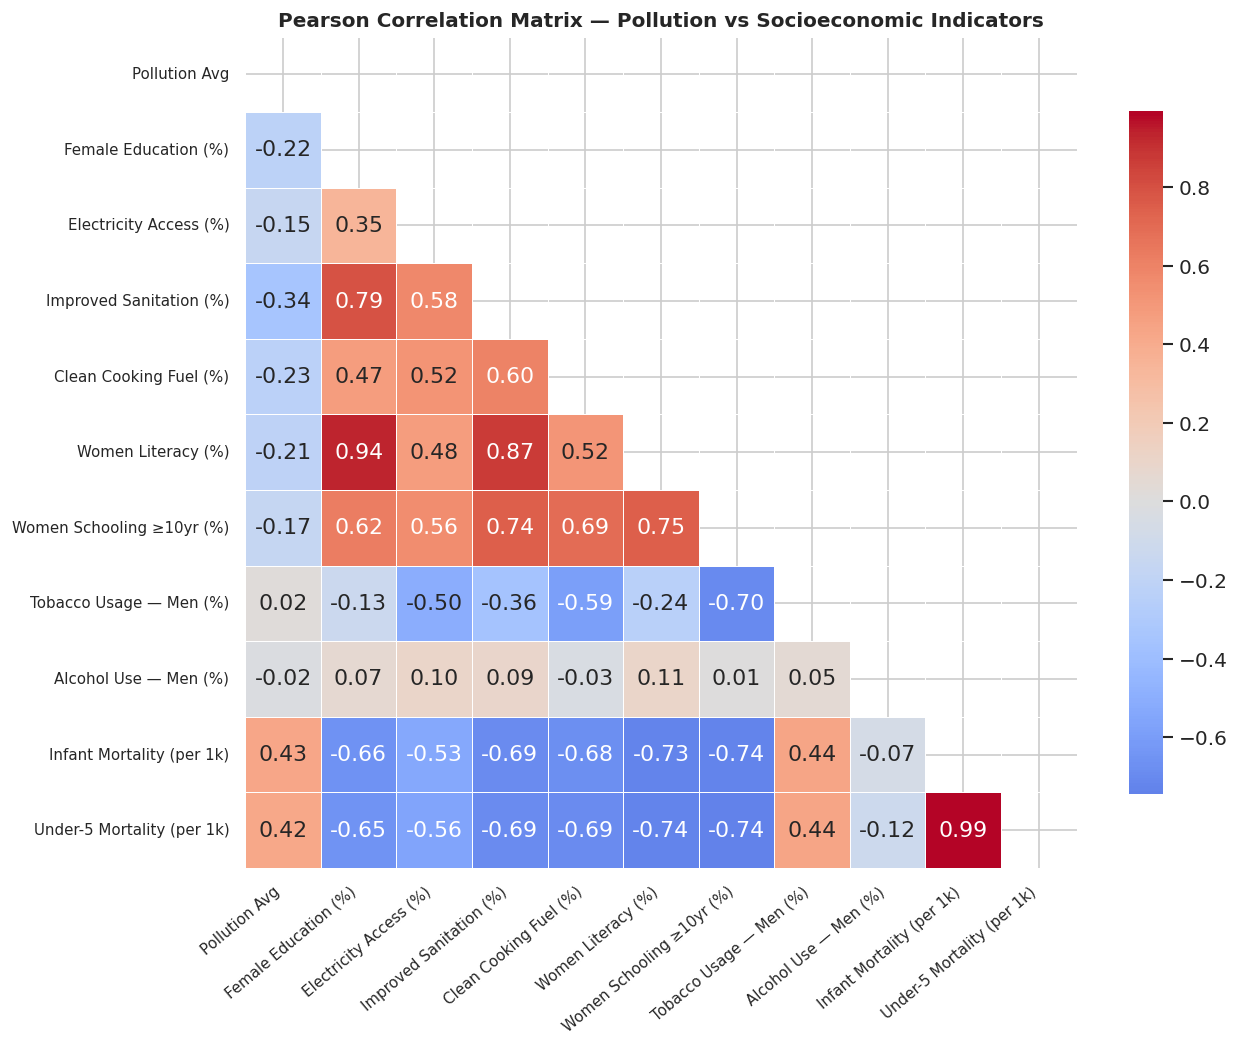
\includegraphics[width=\linewidth]{fig5_correlation_matrix}
  \caption{Pearson correlation matrix --- pollution vs
           socioeconomic indicators (lower triangle; colour
           scale: blue~$=$~negative, red~$=$~positive).}
  \label{fig:corr_matrix}
\end{figure}

\subsection{K-Means Clustering}

The Elbow Method identified $k = 3$ as the optimal cluster
number.
Table~\ref{tab:clusters} summarises cluster profiles.

\begin{table}[htbp]
  \centering
  \caption{K-Means Cluster Profiles (Mean Values, $k=3$)}
  \label{tab:clusters}
  \renewcommand{\arraystretch}{1.1}
  \begin{tabular}{@{}crrrrp{3.0cm}@{}}
    \toprule
    \textbf{C} & \textbf{Poll.} & \textbf{Elec.} & \textbf{San.}
      & \textbf{FEd.} & \textbf{Representative States} \\
    \midrule
    0 & $\sim$47 & 91\% & 72\% & 79\%
      & Delhi, Jharkhand, Haryana, Punjab, Odisha \\
    1 & $\sim$28 & 90\% & 67\% & 74\%
      & Assam, Bihar, Nagaland, Tripura \\
    2 & $\sim$24 & 98\% & 93\% & 88\%
      & Chandigarh, Gujarat, Karnataka, Kerala \\
    \bottomrule
    \multicolumn{6}{@{}l}{\footnotesize
      Poll.~=~Mean Pollution; Elec.~=~Electricity;
      San.~=~Sanitation; FEd.~=~Female Education.}
  \end{tabular}
\end{table}

Cluster~0 groups high-pollution states with moderately
developed infrastructure --- consistent with the
urbanisation-pollution nexus.
Cluster~2 represents states combining lower pollution with
high development indicators, broadly characterising southern
and western India.
Cluster~1 captures north-eastern and eastern states with
moderate-to-lower development and lower pollution, largely
reflecting lower industrial density.
Figure~\ref{fig:clusters} visualises the cluster assignments.

\begin{figure}[htbp]
  \centering
  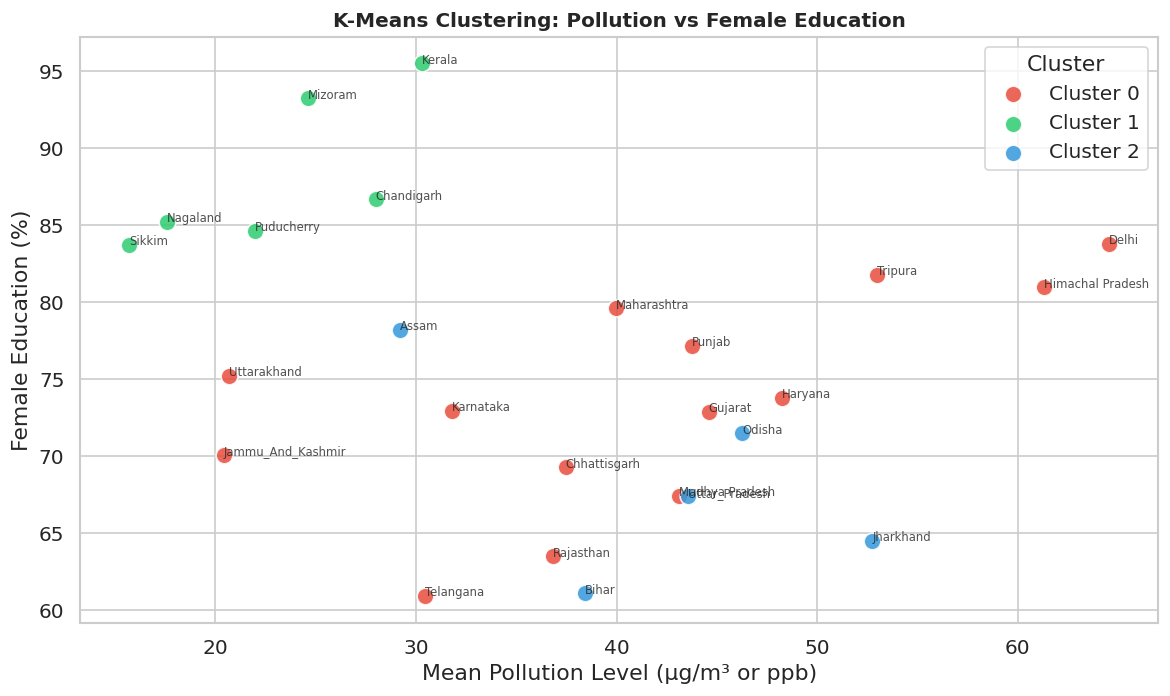
\includegraphics[width=\linewidth]{fig8_kmeans_clusters}
  \caption{K-Means clustering ($k=3$) projected onto the
           Mean Pollution vs.\ Female Education axes.
           Each point represents a state; colours denote
           cluster membership.}
  \label{fig:clusters}
\end{figure}

\subsection{Predictive Modelling}

Table~\ref{tab:models} compares regression model performance
on the held-out test set ($n_{\text{test}} = 6$) and via
five-fold cross-validation.

\begin{table}[htbp]
  \centering
  \caption{Regression Model Performance ($n = 29$, 80/20 split)}
  \label{tab:models}
  \renewcommand{\arraystretch}{1.1}
  \begin{tabular}{@{}lrrrr@{}}
    \toprule
    \textbf{Model} & \textbf{MAE} & \textbf{RMSE}
      & \textbf{Test $R^2$} & \textbf{CV $R^2$} \\
    \midrule
    Linear Regression  & 16.24 & 18.81 & $-0.367$ & $-1.998$ \\
    Ridge Regression   & 15.79 & 18.00 & $-0.253$ & $-1.618$ \\
    \textbf{Random Forest} & \textbf{12.77} & \textbf{15.35}
      & $\mathbf{+0.090}$ & $-1.515$ \\
    Gradient Boosting  & 14.95 & 19.04 & $-0.402$ & $-2.873$ \\
    \bottomrule
  \end{tabular}
\end{table}

All models yield negative CV~$R^2$ values, indicating no
reliable generalisation beyond the training sample.
Random Forest achieves a marginally positive held-out
$R^2$ ($+0.090$), though this reflects the limited test fold
size (six states).
This outcome is a finding in itself:
\emph{socioeconomic features as measured here are
insufficient to reliably predict state-level composite
pollution at $n = 29$}.
A larger longitudinal panel --- incorporating temporal
variation and within-state city-level observations ---
is necessary for meaningful predictive modelling.

Despite poor predictive accuracy, Random Forest feature
importances (Figure~\ref{fig:feat_importance}) provide
exploratory directional insight.
Clean cooking fuel access and electricity access rank highest,
followed by female education and women's literacy.
This is consistent with the understanding that household
energy transition (from biomass to LPG/electricity) directly
reduces particulate emissions, and that states with higher
electrification tend to have greater environmental regulatory
capacity.

\begin{figure}[htbp]
  \centering
  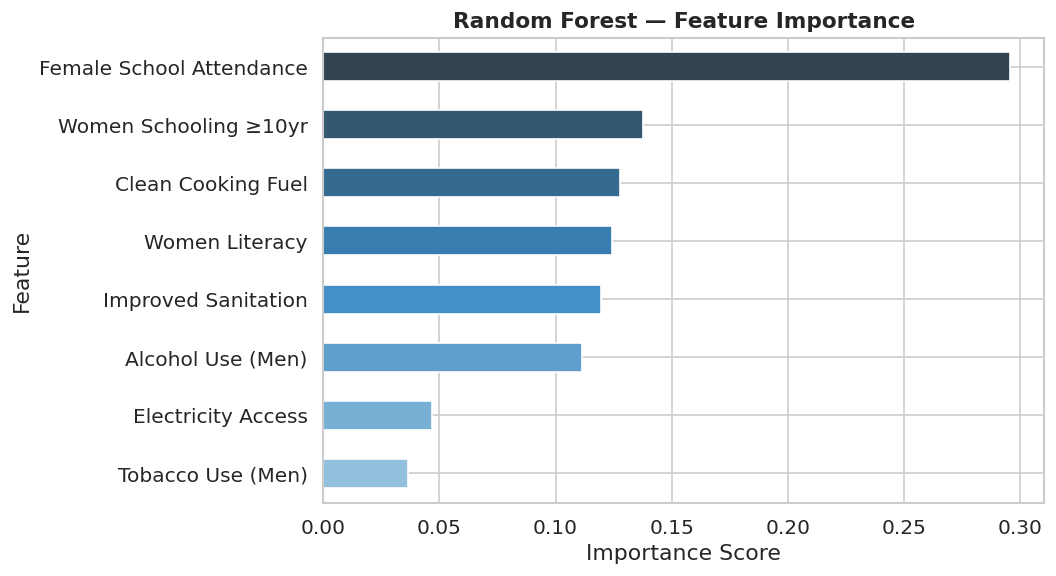
\includegraphics[width=\linewidth]{fig9_feature_importance}
  \caption{Random Forest feature importance scores.
           Higher scores indicate greater influence on the
           predicted state-level mean pollution value.}
  \label{fig:feat_importance}
\end{figure}

% ============================================================
%  5. CONCLUSION
% ============================================================
\section{Conclusion}
\label{sec:conclusion}

This study presents an integrated analysis of CPCB real-time
air quality data and NFHS-5 socioeconomic indicators across
Indian states, contributing a reproducible, multi-method
analytical framework.
The principal findings are:

\begin{enumerate}[leftmargin=*]
  \item \textbf{Particulate matter dominates India's air
        quality burden.}
        Mean PM$_{10}$ and PM$_{2.5}$ concentrations exceed
        WHO guidelines by six- and fifteenfold respectively.
        Northern and eastern states bear a disproportionate
        pollution burden.
  \item \textbf{Child mortality indicators are the only
        statistically significant correlates} of state-level
        pollution exposure (infant mortality: $r = {+}0.45$,
        $p = 0.017$; under-five mortality: $r = {+}0.44$,
        $p = 0.021$).
  \item \textbf{K-Means clustering reveals three distinct
        state profiles:} a high-pollution/moderate-development
        cluster (northern industrial states), a
        lower-pollution/lower-development cluster
        (north-eastern states), and a
        lower-pollution/higher-development cluster
        (southern and western states).
  \item \textbf{Predictive modelling is fundamentally
        constrained} by the small matched sample (29~states).
        No model achieved reliable held-out CV~$R^2$.
  \item \textbf{Clean cooking fuel and electricity access}
        are the most informative exploratory features,
        reinforcing the policy relevance of household energy
        transition programmes (Ujjwala Yojana, Saubhagya)
        as co-benefit strategies for air quality improvement.
\end{enumerate}

\subsection{Limitations}

\begin{itemize}[leftmargin=*]
  \item The merged dataset covers only 29 of 37 NFHS states.
  \item AQI data represents a single cross-sectional snapshot;
        causal inference requires longitudinal panel data.
  \item Temporal alignment between CPCB readings and NFHS-5
        estimates (2019--21) is approximate.
  \item State-level aggregation masks substantial intra-state
        heterogeneity between urban and rural areas.
  \item No direct respiratory health outcome variables
        (e.g., hospital admissions) were available in the
        current datasets.
\end{itemize}

\subsection{Future Work}

\begin{itemize}[leftmargin=*]
  \item Incorporate multi-year CPCB data (2017--present) to
        enable panel regression and trend analysis.
  \item Use city/district-level linkage between CPCB stations
        and NFHS Primary Sampling Units for higher-resolution
        analysis.
  \item Apply spatial regression models (Spatial Lag,
        Geographically Weighted Regression) to account for
        spatial autocorrelation.
  \item Integrate satellite-derived PM$_{2.5}$ data
        (NASA MERRA-2, MODIS) to extend coverage beyond
        ground-monitoring locations.
\end{itemize}

% ============================================================
%  ACKNOWLEDGEMENTS
% ============================================================
\section*{Acknowledgements}
The author thanks the Central Pollution Control Board (CPCB)
and the Ministry of Health and Family Welfare, Government of
India, for making the AQI and NFHS-5 datasets publicly
available on data.gov.in.
The analysis was conducted as part of coursework at
Chandigarh University (B.Tech CSE, UID: 25LBCS1407).

% ============================================================
%  REFERENCES
% ============================================================
\balance
\bibliographystyle{IEEEtran}

\begin{thebibliography}{10}

\bibitem{balakrishnan2019}
K.~Balakrishnan et al.,
``The impact of air pollution on deaths, disease burden, and
life expectancy across the states of India: the Global Burden
of Disease Study 2017,''
\textit{The Lancet Planetary Health}, vol.~3, no.~1,
pp.~e26--e39, 2019.

\bibitem{hei2020}
Health Effects Institute,
\textit{State of Global Air 2020: A Special Report on Global
Exposure to Air Pollution and its Disease Burden},
Boston, MA: HEI, 2020.

\bibitem{kumar2015}
P.~Kumar et al.,
``Real-time sensors for indoor air monitoring and challenges
ahead in deploying them to urban buildings,''
\textit{Science of the Total Environment},
vols.~560--561, pp.~150--159, 2015.

\bibitem{garg2021}
A.~Garg et al.,
``An assessment of air quality over major Indian cities
during COVID-19 lockdown,''
\textit{Urban Climate}, vol.~36, p.~100793, 2021.

\bibitem{landrigan2018}
P.~J.~Landrigan et al.,
``The Lancet Commission on pollution and health,''
\textit{The Lancet}, vol.~391, no.~10119,
pp.~462--512, 2018.

\bibitem{chowdhury2016}
S.~Chowdhury and S.~Dey,
``Cause-specific premature death from ambient PM2.5 exposure
in India: Estimate adjusted for baseline mortality,''
\textit{Environment International}, vol.~91,
pp.~283--290, 2016.

\bibitem{nfhs5}
Ministry of Health and Family Welfare, Government of India,
\textit{National Family Health Survey-5 (NFHS-5), 2019--21:
India Report},
Mumbai: IIPS, 2021.

\bibitem{cpcb2022}
Central Pollution Control Board,
\textit{National Ambient Air Quality Standards (NAAQS) and
AQI Calculation Methodology},
New Delhi: CPCB, 2022.

\bibitem{who2021}
World Health Organization,
\textit{WHO Global Air Quality Guidelines: Particulate Matter
(PM2.5 and PM10), Ozone, Nitrogen Dioxide, Sulfur Dioxide
and Carbon Monoxide},
Geneva: WHO, 2021.

\bibitem{pedregosa2011}
F.~Pedregosa et al.,
``Scikit-learn: Machine learning in Python,''
\textit{Journal of Machine Learning Research}, vol.~12,
pp.~2825--2830, 2011.

\end{thebibliography}

% ============================================================
%  APPENDIX A — Figures
% ============================================================
\appendix
\section{Additional Figures}
\label{app:figures}

\begin{figure}[htbp]
  \centering
  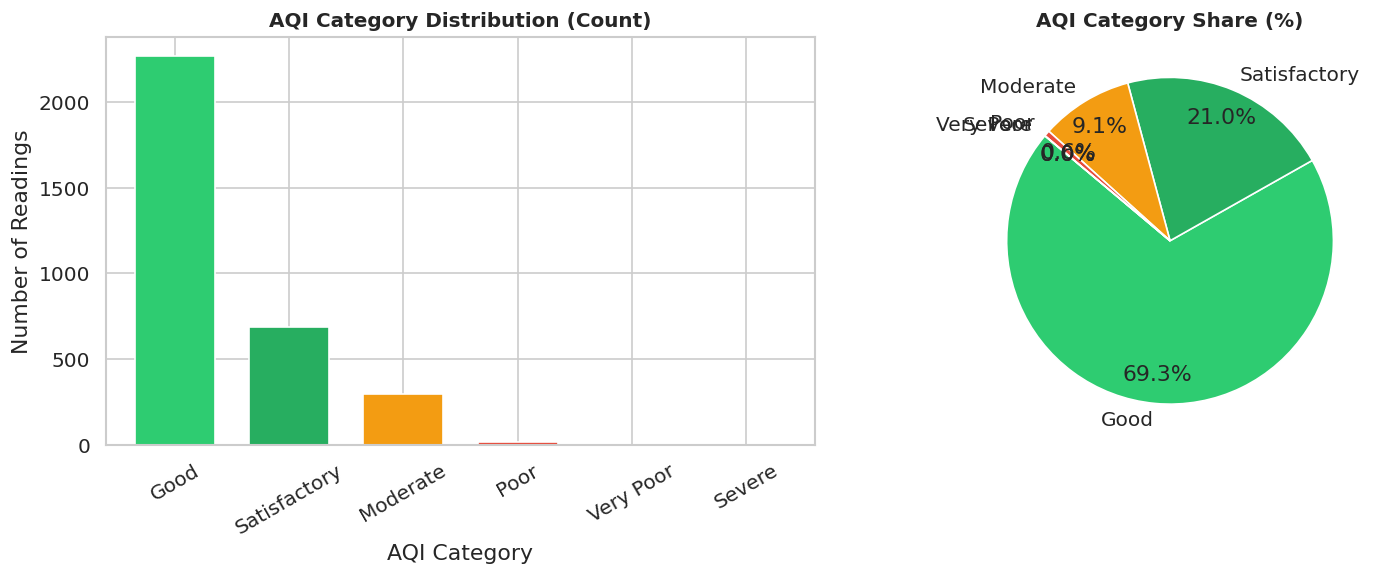
\includegraphics[width=\linewidth]{fig3_aqi_categories}
  \caption{AQI category distribution: (left)~count bar chart;
           (right)~percentage pie chart.}
  \label{fig:aqi_cat}
\end{figure}

\begin{figure}[htbp]
  \centering
  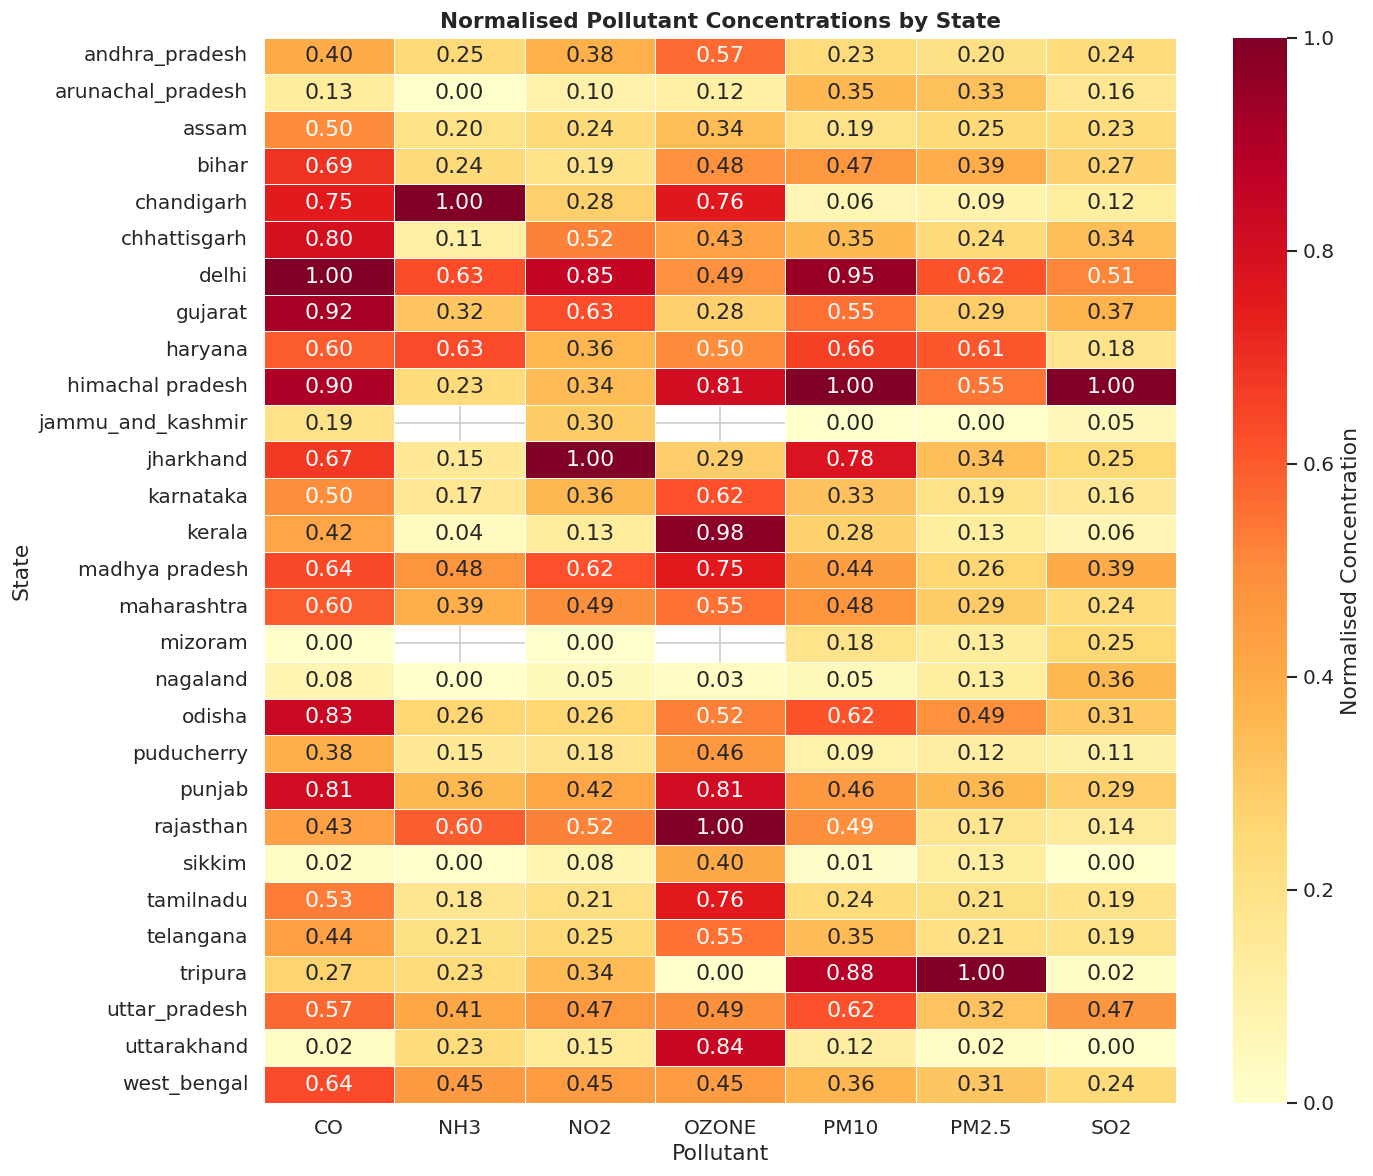
\includegraphics[width=\linewidth]{fig4_state_pollutant_heatmap}
  \caption{Normalised pollutant concentrations by state
           (0--1 scale per pollutant column).}
  \label{fig:heatmap}
\end{figure}

\begin{figure}[htbp]
  \centering
  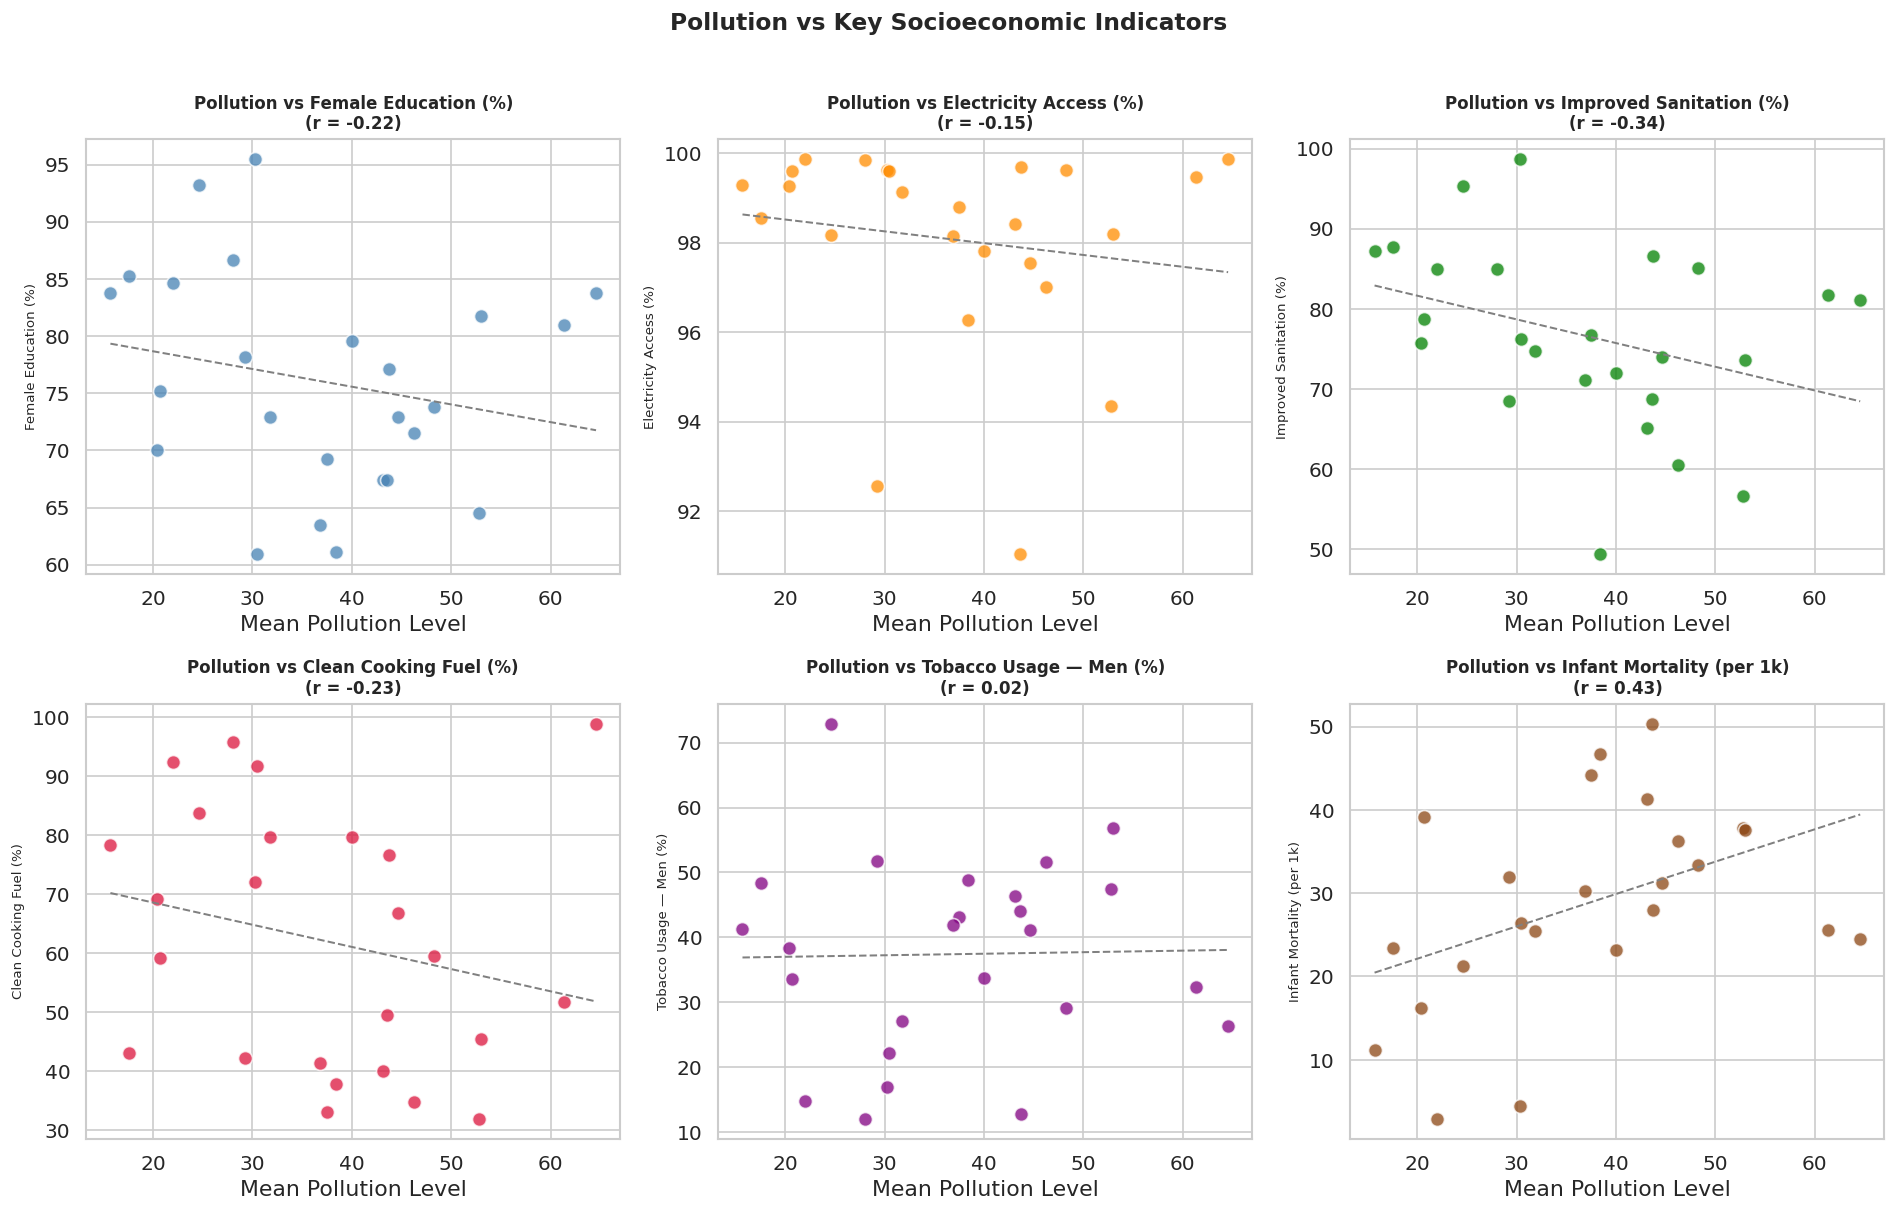
\includegraphics[width=\linewidth]{fig6_scatter_plots}
  \caption{Scatter plots --- state-level mean pollution vs
           key socioeconomic indicators with OLS trend lines.}
  \label{fig:scatter}
\end{figure}

\begin{figure}[htbp]
  \centering
  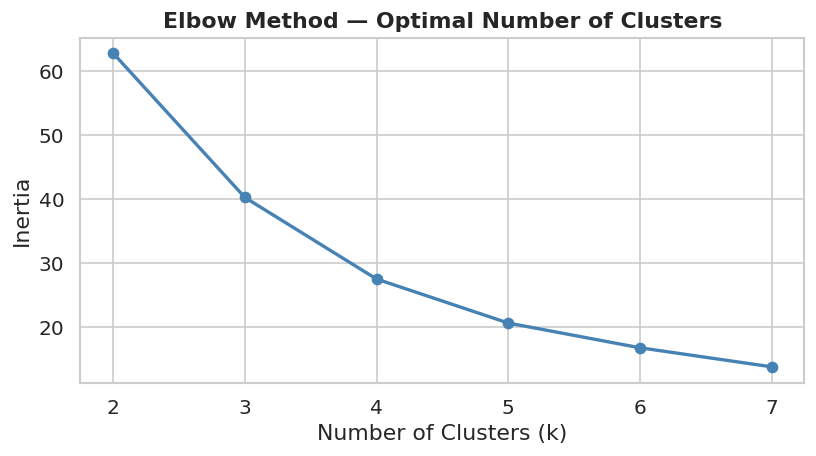
\includegraphics[width=0.75\linewidth]{fig7_elbow}
  \caption{Elbow Method for K-Means: inertia vs.\ number
           of clusters. The elbow at $k=3$ justifies the
           chosen cluster count.}
  \label{fig:elbow}
\end{figure}

\begin{figure}[htbp]
  \centering
  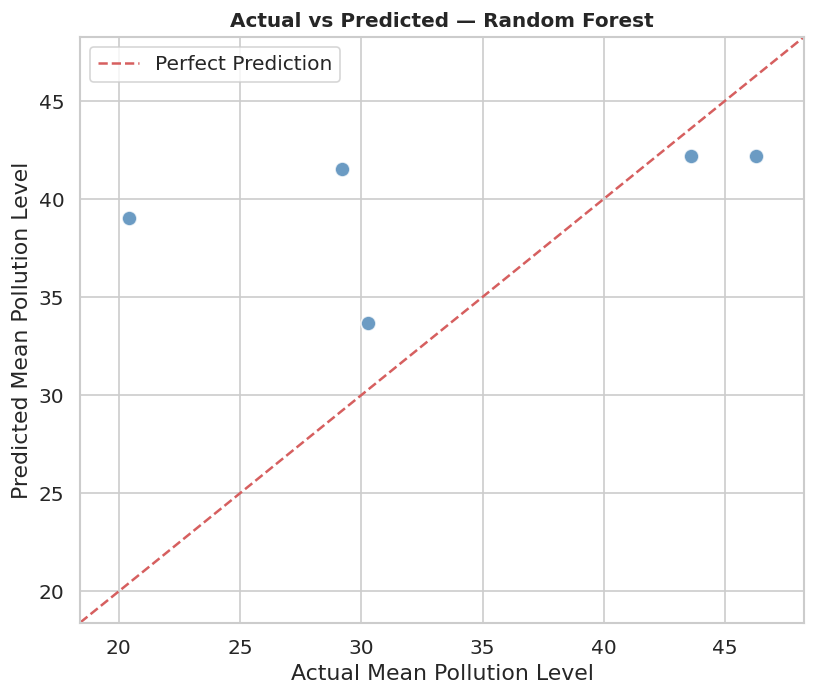
\includegraphics[width=\linewidth]{fig10_actual_vs_predicted}
  \caption{Actual vs.\ predicted mean pollution level for
           the best model (Random Forest).
           The dashed red line represents perfect prediction.}
  \label{fig:actual_pred}
\end{figure}

\begin{figure}[htbp]
  \centering
  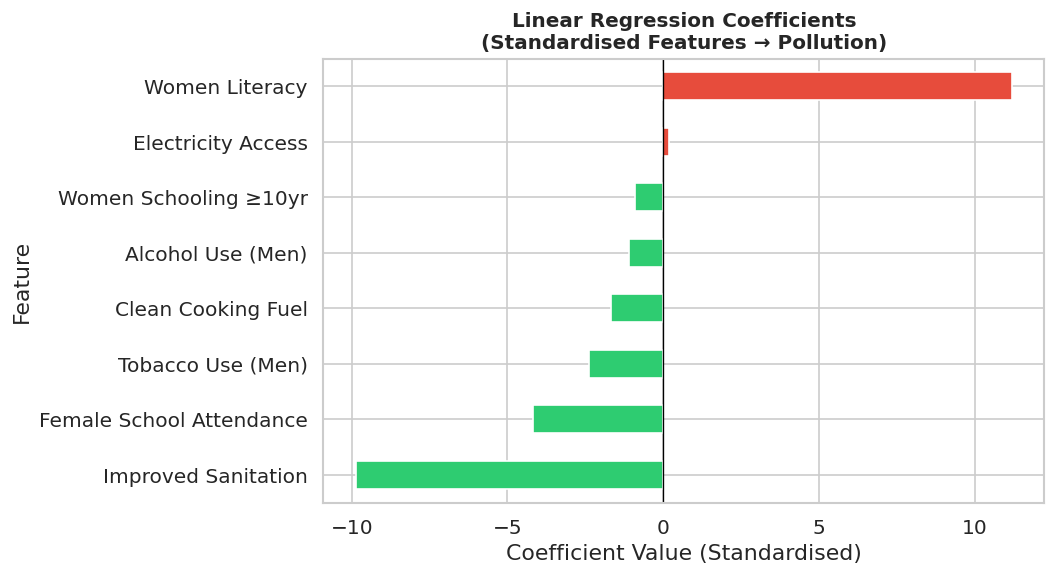
\includegraphics[width=\linewidth]{fig11_lr_coefficients}
  \caption{Linear Regression standardised coefficients.
           Red bars indicate features positively associated
           with pollution; green bars indicate negative
           associations.}
  \label{fig:lr_coeff}
\end{figure}

% ============================================================
%  APPENDIX B — Reproducibility
% ============================================================
\section{Reproducibility}
\label{app:repro}

All analyses are fully reproducible using the accompanying
Jupyter Notebook \texttt{CPCB\_AQI\_Analysis.ipynb} and the
two raw data files \texttt{aqi.csv} and \texttt{health.xls}.
Python dependencies are listed in \texttt{requirements.txt}.
To reproduce:

\begin{lstlisting}[language=bash, caption={Reproducing the analysis}]
# 1. Install dependencies
pip install -r requirements.txt

# 2. Execute the notebook
jupyter nbconvert --to notebook \
  --execute CPCB_AQI_Analysis.ipynb \
  --output CPCB_AQI_Analysis_executed.ipynb
\end{lstlisting}

\noindent The notebook produces all 11 figures
(Figures~\ref{fig:pollutant_dist}--\ref{fig:lr_coeff})
automatically and prints all numerical results reported in
this paper.

\end{document}
